% THIS DOCUMENT IS FOLLOWS THE VOLERE TEMPLATE BY Suzanne Robertson and James Robertson
% ONLY THE SECTION HEADINGS ARE PROVIDED
%
% Initial draft from https://github.com/Dieblich/volere
%
% Risks are removed because they are covered by the Hazard Analysis
\documentclass[12pt]{article}
\pdfinfoomitdate=1
\pdftrailerid{}

\usepackage{booktabs}
\usepackage{tabularx}
\usepackage{hyperref}
\usepackage{enumitem}
\hypersetup{
    bookmarks=true,         % show bookmarks bar?
    colorlinks=true,        % false: boxed links; true: colored links
    linkcolor=red,          % color of internal links (change box color with linkbordercolor)
    citecolor=green,        % color of links to bibliography
    filecolor=magenta,      % color of file links
    urlcolor=cyan           % color of external links
}

\newcommand{\lips}{\textit{Insert your content here.}}

%% Comments

\usepackage{color}

% \newif\ifcomments\commentstrue %displays comments
\newif\ifcomments\commentsfalse %so that comments do not display

\ifcomments
  \newcommand{\authornote}[3]{\textcolor{#1}{[#3 ---#2]}}
  \newcommand{\todo}[1]{\textcolor{red}{[TODO: #1]}}
\else
  \newcommand{\authornote}[3]{}
  \newcommand{\todo}[1]{}
\fi

\newcommand{\wss}[1]{\authornote{magenta}{SS}{#1}}
\newcommand{\plt}[1]{\authornote{cyan}{TPLT}{#1}} %For explanation of the template
\newcommand{\an}[1]{\authornote{cyan}{Author}{#1}}

%% Common Parts

\newcommand{\progname}{RoCam} % PUT YOUR PROGRAM NAME HERE
\newcommand{\authname}{Team \#3, SpaceY
    \\ Zifan Si
    \\ Jianqing Liu
    \\ Mike Chen
    \\ Xiaotian Lou} % AUTHOR NAMES                  

\usepackage{hyperref}
\hypersetup{colorlinks=true, linkcolor=blue, citecolor=blue, filecolor=blue,
    urlcolor=blue, unicode=false}
\urlstyle{same}

\usepackage{indentfirst}
\usepackage{graphicx}

\usepackage{titling}

\pretitle{\begin{center}
\includegraphics[width=0.5\textwidth]{../../assets/logo/black.png}\\[0.75em]\LARGE}
        \posttitle{\par\end{center}}

\usepackage[letterpaper, portrait, margin=1in]{geometry}

\usepackage{placeins}

\begin{document}

\title{Software Requirements Specification for \progname: High Performance Vision-Guided Rocket Tracker}
\author{\authname}
\date{\today}

\maketitle

~\newpage

\tableofcontents

~\newpage

\section*{Revision History}

\begin{tabularx}{\textwidth}{p{3cm}p{2cm}X}
  \toprule {\textbf{Date}} & {\textbf{Version}} & {\textbf{Notes}} \\
  \midrule
  Date 1                   & 1.0                & Notes            \\
  Date 2                   & 1.1                & Notes            \\
  \bottomrule
\end{tabularx}

~\\

~\newpage
\section{Purpose of the Project}
\subsection{User Business}

Student and amateur rocketry teams, launch organizers, and technical judges
need reliable, high-fidelity visual evidence of rocket flights to analyze
staging behavior, parachute deployment, and flight anomalies that occur at
extreme speeds and altitudes. Manual camera operation is impractical in these
conditions, and existing tools (manual PTZ/GPS-centric systems) often fail to
maintain visual lock on small, fast-moving vehicles. This project addresses
this gap with an autonomous, vision-based tracking camera designed to lock onto
and follow rockets from launch through landing, providing real-time and
recorded footage for post-flight analysis and event operations.

\subsection{Goals of the Project}

\textbf{Purpose:}

Develop a software+hardware stack (the system) that is able to command a gimbal
with a camera mounted on it to track and record model rocket launches.

\textbf{Advantage:}

The system provides insights into the flight performance by having high quality
flight footage.

\textbf{Measure:}

Deploy the system at small-scale model rocket launch site with apogee less than
200 meters. The system should provide higher quality flight footage than the
manual camera operation.

\section{Stakeholders}

\subsection{Client}

The client of this project is McMaster Rocketry Team. they are the primary end
users who will deploy the system during launches.

\subsection{Customer}

Apart from our client, we also identified the following customers that may be
interested in using the project:

\begin{enumerate}
  \item \textbf{Model Rocketry Event Organizers}: Benefit from
        reliable tracking for live streaming of rocket flights.
  \item \textbf{Model Rocketry Safety Officers}: Benefit from
        live monitoring of parachute deployment and landing location
        of the rockets.
  \item \textbf{Aerospace Engineers and Researchers}: Benefit from
        high-quality flight footage to validate models, improve rocket
        designs, and support experimental research.
\end{enumerate}

\subsection{Other Stakeholders}

\begin{enumerate}
  \item \textbf{Dr. Shahin Sirouspour (Supervisor)}: Provides
        technical guidance, project oversight, and mentorship. Ensures
        the project aligns with academic standards, engineering best
        practices, and capstone deliverable expectations.
\end{enumerate}

\subsection{Hands-On Users of the Project}

Here are the users that will be interacting with the product directly.

\textbf{Role: Camera Operator}

The camera operator controls the system through the UI, starts/stops
recordings, manages tracking states, and monitors preview. The camera operator
is assumed to have a decent level of familiarity with technology, and have been
trained on the use of the product.

\textbf{Role: Live Stream Technician}

The live stream technician manages the video feed from the system to the live
streaming equipments. The live stream technician is assumed to have a high
level of familiarity with live streaming software and hardware.

\textbf{Role: Flight Performance Analyst}

The flight performance analyst is a member of the rocketry team that
reconstructs flight profiles from sensor data and camera footage to understand
how the rocket behaves during ascent and recovery. The flight performance
analyst is assumed to have a high level of familiarity with rocket flight
dynamics and software used for analysis.

\textbf{Role: Live Stream / Recordings Viewers}

People who view the live stream or recorded videos. They can be anyone from the
general public that are interested in the launch, or the team members
themselves. They are assumed to have a basic level of familiarity with
technology.

\subsection{Personas}

\subsubsection*{Alexis Andrade}

\textbf{Age}: 28

\textbf{Role}: Camera Operator

Alexis works as an industrial automation technician in Hamilton, Ontario, where
she designs and maintains robotic assembly systems for a manufacturing firm.
Outside of work, her real passion lies in high-speed imaging and experimental
photography — a hobby that naturally led her to volunteer as a staff camera
operator at university rocketry competitions. She loves the mix of engineering
precision and adrenaline that comes with capturing a successful rocket launch.

She lives with her partner and their energetic border collie, Pixel. Alexis
spends her weekends hiking the Bruce Trail, refurbishing vintage lenses, or
volunteering at local maker fairs. Her favorite food is falafel, and she always
packs a thermos of strong coffee for early launch mornings. She listens to
synthwave and retro electronic music on long drives to test sites, finding it
helps her stay calm and focused.

Alexis is confident with technology but prefers systems that are reliable and
straightforward. She values hands-on work, hates clunky software interfaces,
and believes in simplicity over flashiness. “If I need a manual,” she likes to
say, “the interface is wrong.” Her cool temperament and technical precision
make her a trusted member of the launch operations crew.

\subsubsection*{Brandon Brooks}

\textbf{Age}: 23

\textbf{Role}: Flight Performance Analyst

Brandon is in his final year of mechanical engineering at a Canadian university
and serves as a flight performance analyst for his rocketry team. His specialty
is reconstructing flight profiles from sensor data and camera footage to
understand how the rocket behaves during ascent and recovery. He joined the
team for the engineering challenge but stayed because he loves the mix of
theory, experimentation, and teamwork.

Originally from Calgary, Brandon now lives in a small off-campus apartment
filled with model rockets, whiteboards, and a curious cat named Fourier. He's
known for his patience and meticulous documentation — traits that make him the
go-to person for post-launch analysis. When he's not studying or coding MATLAB
scripts, he's cooking ramen, taking photos, or biking along Lake Ontario.

Brandon listens to ambient and post-rock while he works, loves strong coffee,
and dislikes chaotic testing days where data logging gets overlooked. His
attitude toward technology is analytical but practical: he values transparency,
well-documented systems, and data that “speaks for itself.” For him, every
successful flight is a story written in numbers and motion.

\subsubsection*{Christopher Chou}

\textbf{Age}: 59

\textbf{Role}: Event Organizer / Live Stream Technician

Christopher is a retired broadcast engineer who spent three decades working in
television production for CBC Toronto. After retirement, he moved to Burlington
and found a new passion in volunteer work, helping organize live streams and
event logistics for student rocketry competitions. For him, it's the perfect
blend of his lifelong love of broadcasting and his fascination with aerospace
technology.

He's married with two grown children who live abroad, and he often jokes that
the rocketry community has become his “third family.” Christopher loves cooking
Cantonese comfort food — especially steamed dumplings and congee — and enjoys
jazz and classic rock in equal measure. He spends his spare time restoring old
audio equipment, gardening, and taking long weekend drives along the Niagara
Escarpment.

Christopher's approach to technology is deeply pragmatic: he respects
automation but insists that every system should have a manual override. He
likes tidy wiring, clear documentation, and software that doesn't crash
midstream. He dislikes unnecessary complexity and “updates that fix what wasn't
broken.” To younger team members, he's both a mentor and the steady hand who
keeps the broadcast running when chaos hits.
\subsection{Priorities Assigned to Users}

\textbf{Key Users}: Camera Operator, Live Stream Technician

\textbf{Secondary User}: Flight Performance Analyst, Live Stream / Recordings Viewers, Event Organizer

\subsection{User Participation}

Through out the development process, the development team will continue to
iterate on the requirements based on feedback from these users:

\begin{enumerate}
  \item \textbf{Camera Operator}: At least three field tests will be conducted
        to gather feedback from the camera operator. Each field test will last
        half a day to a day.
  \item \textbf{Live Stream Technician}: At least two meetings will be conducted
        to gather feedback from the live stream technician.
\end{enumerate}

\subsection{Maintenance Users and Service Technicians}

Due to the nature of this project as a capstone requirement, there are
currently no expected maintenance users.

\section{Mandated Constraints}
\subsection{Solution Constraints}

\begin{enumerate}[label=MD-SL \arabic*., wide=0pt, leftmargin=*]
  \item \emph{The system must be hands-off (autonomous) from rocket ignition through landing.}\\[2mm]
        {\bf Rationale:} During live launches, human operators must prioritize range safety and situational awareness\\
        {\bf Fit Criterion:} Once ready, no manual inputs are necessary for the nominal operation of the system until a declared “landed/clear” signal from the mission control.

  \item \emph{The system must be remote controllable.}\\[2mm]
        {\bf Rationale:} The system may need to be positioned inside hazardous zones (launch pad, ballistic landing areas) or at distant vantage points with no safe operator access during the countdown and flight.\\
        {\bf Fit Criterion:} The system should be able to perform all the product use cases with no physical interaction at the camera site once deployed.

  \item \emph{The system must output a live video stream via HDMI.}\\[2mm]
        {\bf Rationale:} The customer's live streaming equipments accept HDMI as the integration standard, alternative connectors would require additional adapters.\\
        {\bf Fit Criterion:} The system should be able to output a live video stream via HDMI, confirmed by connecting a monitor to the system.

  \item \emph{The system must provide a flexible interface for gimbal hardware.}\\[2mm]
        {\bf Rationale:} Different deployment contexts require different hardware: lighter gimbal for algorithm development and small scale launches, or full-scale gimbal for large scale launches with telescoping lens.\\
        {\bf Fit Criterion:} A documented gimbal interface for both hardware and software.
\end{enumerate}

\subsection{Implementation Environment of the Current System}

There are no constrains on the hardware platform the system need to use.

\subsection{Partner or Collaborative Applications}

The system is expected to be used with a gimbal with a camera mounted on it.
The system will command the gimbal to track and record model rocket launches.

\subsection{Off-the-Shelf Software}

There are no constrains on the off-the-shelf software the system need to use.

\subsection{Anticipated Workplace Environment}

The system should be designed to operate in a large-scale outdoor launch
environment, for example, the Launch Canada launch site in Timmins, Ontario, Or
Spaceport America in New Mexico.

The tracking camera will be operated at outdoor launch sites, typically in wide
open fields or designated rocket ranges. Launches occur only under clear, sunny
conditions with few or no clouds.

Additionally, users often wear hearing protection devices to mitigate high
acoustic noise from tools, filling tanks, and generators.

Launch sites are typically in a remote area, with limited or no internet
access.

\subsection{Schedule Constraints}

\begin{enumerate}[label=SCHD \arabic*., wide=0pt, leftmargin=*]
  \item \emph{The project shall be completed by April 2026, with
          interim deadlines for key milestones such as Proof of Concept
          (November 2025) and the final demonstration (March 2026).}\\[2mm]
        {\bf Rationale:} These deadlines are based on the academic
        timeline and the expectations of the capstone course.\\
        {\bf Fit Criterion:} All project components must be completed and
        fully functional by the final demonstration in March 2026.
\end{enumerate}

\subsection{Budget Constraints}

\begin{enumerate}[label=BDGT \arabic*., wide=0pt, leftmargin=*]
  \item \emph{The project shall not exceed the budget of 500CAD}\\[2mm]
        {\bf Rationale:} Limited by the capstone project requirement\\
        {\bf Fit Criterion:} The sum of the costs of the hardware components required for the project must be less than 500CAD.
\end{enumerate}

\subsection{Enterprise Constraints}

\begin{enumerate}[label=ENTP \arabic*., wide=0pt, leftmargin=*]
  \item \emph{The product shall be built to comply with the standards
          of McMaster University's capstone project requirements and
          academic integrity policies.}\\[2mm]
        {\bf Rationale:} The project is part of the university's
        curriculum and must adhere to its standards.\\
        {\bf Fit Criterion:} The product must meet the requirements
        specified by the course syllabus and project advisor.
\end{enumerate}

\section{Naming Conventions and Terminology}
\subsection{Glossary of All Terms, Including Acronyms, Used by Stakeholders
  involved in the Project}

\begin{enumerate}
  \item \textbf{The System}: The software+hardware stack developed for this project that is able to command a gimbal with camera mounted on it to track and record a rocket flight. (the gimbal and the camera are not a part of the system)
  \item \textbf{Gimbal}: A gimbal is a motorized device that rotates based on the commands sent to it.
  \item \textbf{Rocket}: Refers to a model rocket.
  \item \textbf{Ascent}: The stage in a model rocket flight where the rocket is ascending.
  \item \textbf{Recovery}: The stage in a model rocket flight where the rocket has reached its apogee and is descending.
\end{enumerate}

\section{Relevant Facts And Assumptions}
\subsection{Relevant Facts}

None.

\subsection{Business Rules}

None.

\subsection{Assumptions}

\begin{enumerate}
  \item We assume the system will not be connected to the public internet. Thus no
        authentication is required.
  \item We assume the system will only be physically accessed by authorized personnel.
  \item We assume the gimbal connected to the system has adequate performance to track
        the rocket. (For example, it can turn fast enough and has enough range of
        motion.)
  \item We assume 110V AC power is available at the launch site.
  \item We assume it will always be sunny at the launch site, because the launch would
        be cancelled in case of bad weather.
\end{enumerate}

\section{The Scope of the Work}
\subsection{The Current Situation}

Currently, the process of recording and analyzing rocket flights relies on
manual camera operators positioned at safe distances from the launch pad. These
operators attempt to visually follow the rocket during ascent and descent using
consumer or semi-professional video cameras mounted on tripods or pan-tilt
systems.

This approach suffers from several limitations:

\textbf{Accuracy:} Human reaction time and limited field of view make it nearly
impossible to keep fast-moving rockets (often exceeding Mach speeds) centered
in frame. The footage is frequently lost during liftoff or staging events,
leaving gaps in post-flight analysis.

\textbf{Safety Constraints:} Because a human operator must be physically present, camera
placement is restricted to safe zones, which may not provide optimal viewing
angles. Cameras cannot always be positioned where the best line-of-sight
exists.

\textbf{Operational Overhead:} Each launch requires trained operators, setup time, and
coordination with the launch control team. Fatigue, stress, and environmental
conditions (sun glare, wind, dust) further degrade performance.

\textbf{Data Quality:} The video produced by manual operators is often shaky,
inconsistently framed, and lacking synchronization with other flight data
(e.g., telemetry or gimbal angle). This reduces its value for engineering
analysis and competition reporting.

\subsection{The Context of the Work}

\hyperref[img:context-of-work]{Figure 1} identifies the scope of the
investigation necessary in order to discover the requirements related to the
work of tracking rockets. The model shows the detailed area of investigation
and how it connects to the adjacent systems.

\FloatBarrier
\begin{figure}[h]
  \centering
  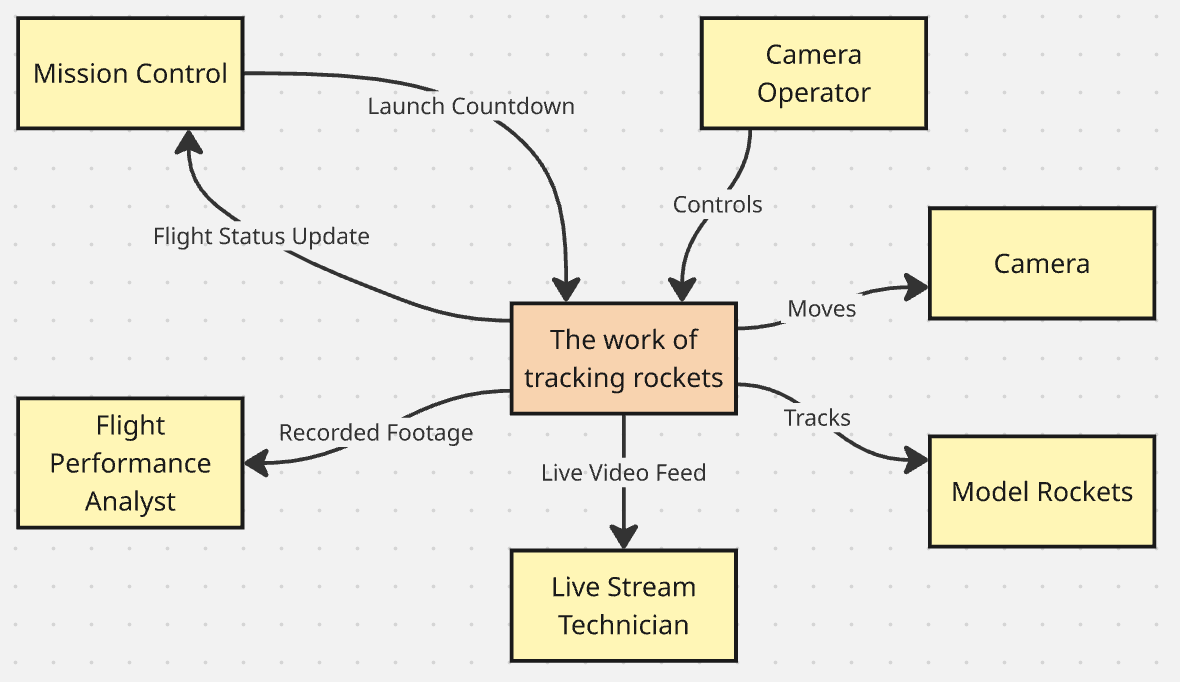
\includegraphics[width=\textwidth,height=\textheight,keepaspectratio]{../Images/context_of_work.png}
  \caption{Context of Work Diagram}
  \label{img:context-of-work}
\end{figure}
\FloatBarrier

\subsection{Work Partitioning}

The \hyperref[tab:work-part]{Table 1} identifies all business events happening
in the real world that affect the work of tracking rockets.

\begin{table}[H]
  \centering
  \setlength\extrarowheight{5mm}
  \begin{tabularx}{\textwidth}{cp{1.5in}X}
    \toprule \textbf{No.} & \textbf{Event Name}                                  &
    \textbf{Input / Output}                                                        \\
    \midrule
    BUC 1                 & Output live video                                    &
    (in) Video feed from camera \newline
    (out) Transmitting the video to the live stream
    \\
    BUC 2                 & Launch countdown starts                              &
    (in) Vocal count down from Mission Control \newline
    (out) Start recording the rocket flight
    \\
    BUC 3                 & Rocket takes flight                                  &
    (in) Video feed from camera \newline
    (out) Keeps pointing the camera to the rocket
    \\
    BUC 4                 & Rocket completes flight                              &
    (in) Video feed from camera \newline
    (out) Stop tracking the rocket \newline
    (out) Save the video  \newline
    (out) Update mission control on flight status
    \\
    BUC 5                 & Flight performance analyst wants to view the footage &
    (in) Request from Flight performance analyst \newline
    (out) Exported video files and logs
    \\
    \bottomrule
  \end{tabularx}
  \caption{Work Partitioning of System}
  \label{tab:work-part}
\end{table}

\subsection{Specifying a Business Use Case (BUC)}

Each event listed in \hyperref[tab:work-part]{Table 1} is expanded into an
individual business use case (BUC) which describes business logic in detail.

~\\

\textbf{BUC 1: Output live video.}

\textbf{Trigger:} None, always active.

\textbf{Interested Stakeholders:} Model Rocketry Event Organizers

\textbf{Preconditions:} Camera is powered on.

\textbf{Main Flow of Steps:}
\begin{enumerate}
  \item The camera operator connect the camera to the live streaming equipments.
\end{enumerate}

\textbf{Outcome:} The live stream receives a video feed from the camera.

~\\

\textbf{BUC 2: Launch countdown starts.}

\textbf{Trigger:} Mission Control begins the countdown to launch.

\textbf{Interested Stakeholders:} Model Rocketry Event Organizers.

\textbf{Preconditions:} Camera is powered on and ready to record.

\textbf{Main Flow of Steps:}
\begin{enumerate}
  \item The camera operator points the camera to the rocket
  \item The camera operator starts recording.
\end{enumerate}

\textbf{Outcome:} Recording of the rocket flight is started.

~\\

\textbf{BUC 3: Rocket takes flight.}

\textbf{Trigger:} Rocket ignition and liftoff are observed.

\textbf{Interested Stakeholders:} Model Rocketry Event Organizers, Aerospace Engineers and Researchers.

\textbf{Preconditions:} Camera is pointing at the rocket and recording.

\textbf{Main Flow of Steps:}
\begin{enumerate}
  \item The camera operator keeps pointing the camera to the rocket.
  \item If the rocket stages, the camera operator points the camera to the next stage.
\end{enumerate}

\textbf{Outcome:} The camera remains pointed at the rocket throughout the flight.

~\\

\textbf{BUC 4: Rocket completes flight.}

\textbf{Trigger:} Rocket landing is observed.

\textbf{Interested Stakeholders:} Model Rocketry Event Organizers, Model Rocketry Safety Officers.

\textbf{Preconditions:} Camera is pointing at the rocket and recording.

\textbf{Main Flow of Steps:}
\begin{enumerate}
  \item The camera operator confirms end of flight based on callout or observation.
  \item The camera operator ends the recording.
  \item The camera operator stops pointing the camera to the rocket.
  \item The camera operator communicates the flight status to Mission Control.
\end{enumerate}

\textbf{Outcome:} Video and logs are safely stored and the flight status is communicated to Mission Control.

~\\

\textbf{BUC 5: Flight performance analyst wants to view the footage.}

\textbf{Trigger:} Flight performance analyst requests to view the footage.

\textbf{Interested Stakeholders:} Aerospace Engineers and Researchers.

\textbf{Preconditions:} None.

\textbf{Main Flow of Steps:}
\begin{enumerate}
  \item The flight performance analyst provides date and time of the flight.
  \item The camera operator looks up the flight in the database.
  \item If the flight is found, the camera operator exports the video files and logs.
  \item If the flight is not found, the camera operator informs the flight performance
        analyst that the flight is not found.
\end{enumerate}

\textbf{Outcome:} The flight performance analyst receives the video files and logs.

\section{Business Data Model and Data Dictionary}
\subsection{Business Data Model}

The business data model consists of a list of launches, and for each launch,
the video footage and logs associated with the launch.

\FloatBarrier
\begin{figure}[h]
  \centering
  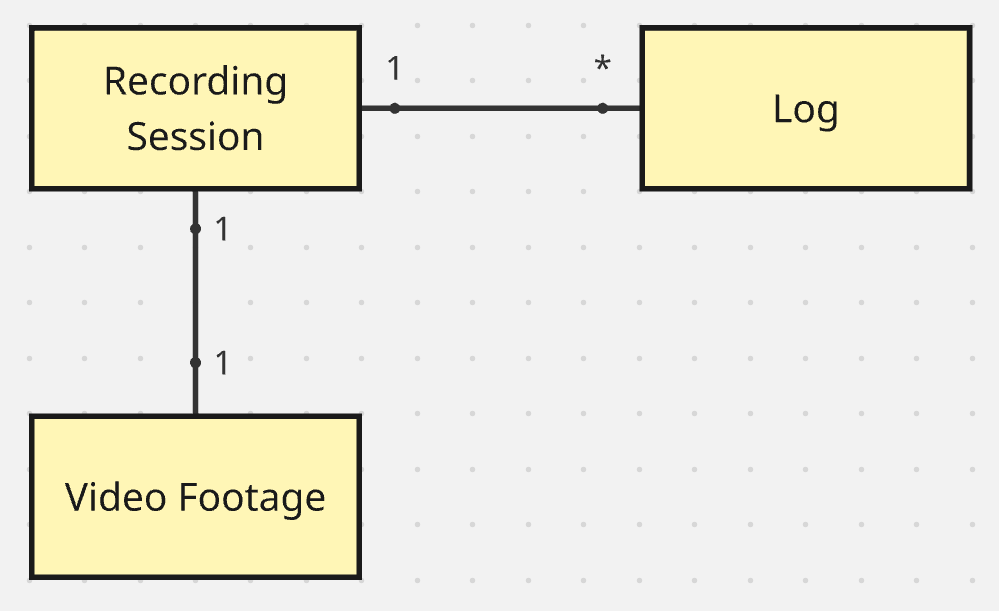
\includegraphics[width=\textwidth,height=\textheight,keepaspectratio]{../Images/business_data_model.png}
  \caption{Business Data Model}
  \label{img:business-data-model}
\end{figure}
\FloatBarrier

\subsection{Data Dictionary}
\lips

\section{The Scope of the Product}
\subsection{Product Boundary}

The product boundary defines which parts of the work are handled by the system
and which parts remain the responsibility of human actors.

In \hyperref[img:product-boundary]{Figure 3}, The product use cases (PUCs) are
the ellipses inside the boundary. Each PUC is labeled with one or more BUCs
that it came from.

\FloatBarrier
\begin{figure}[h]
  \centering
  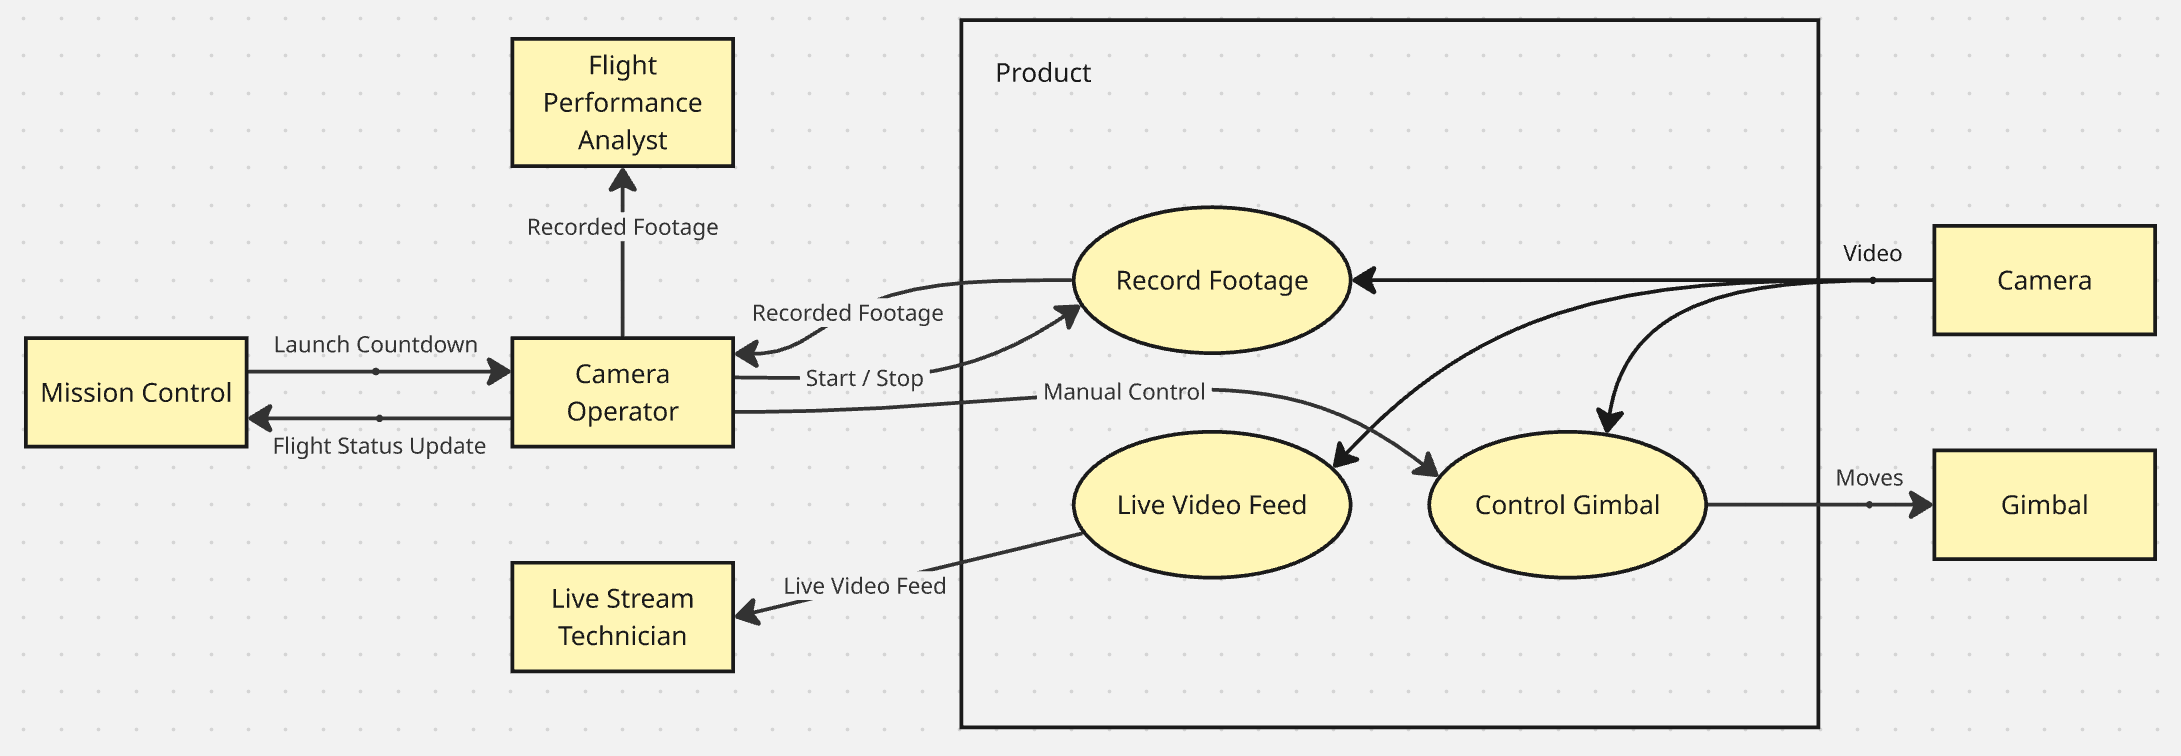
\includegraphics[width=\textwidth,height=\textheight,keepaspectratio]{../Images/product_boundary.png}
  \caption{Product Boundary}
  \label{img:product-boundary}
\end{figure}
\FloatBarrier

\subsection{Product Use Case Table}

The following \hyperref[tab:product-use-case-table]{Table 2} summarizes the
primary use cases of the system.

\begin{table}[H]
  \centering
  \setlength\extrarowheight{5mm}
  \begin{tabularx}{\textwidth}{p{0.4in}p{0.4in}p{1.25in}p{1in}X}
    \toprule \textbf{BUC No.}       & \textbf{PUC No.}        & \textbf{PUC Name}              &
    \textbf{Actors}                 & \textbf{Input / Output}                                    \\
    \midrule
    1                               & 1                       & Live video output              &
    Camera, Live Stream Technician
                                    &
    (in) Video feed from camera \newline
    (out) Live video output                                                                      \\
    2                               & 2.1                     & Point camera to rocket         &
    Camera Operator, Camera, Gimbal
                                    &
    (in) Manual gimbal adjustment commands from camera operator \newline
    (out) Movement commands to the gimbal                                                        \\
    2                               & 2.2                     & Start video recording          &
    Camera Operator, Camera
                                    &
    (in) Start video recording command \newline
    (out) Video recording started                                                                \\
    2                               & 2.3                     & Start tracking rocket          &
    Camera Operator, Camera, Gimbal
                                    &
    (in) Start tracking rocket command \newline
    (out) System in armed state                                                                  \\

    3                               & 3                       & Automated rocket tracking      &
    Camera, Gimbal                  &
    (in) Video feed from camera \newline
    (out) Movement commands to gimbal                                                            \\
    4                               & 4.1                     & Stop video recording           &
    Camera Operator, Camera         &
    (in) Stop video recording command \newline
    (out) Video recording stopped and saved                                                      \\
    4                               & 4.2                     & Stop tracking rocket           &
    Camera Operator, Camera, Gimbal &
    (in) Stop tracking rocket command \newline
    (out) Gimbal stops moving \newline
    (out) System in idle state                                                                   \\
    5                               & 5                       & View recorded footage and logs &
    Camera Operator                 &
    (in) request to download footage and logs \newline
    (out) Footage and logs downloaded                                                            \\

    \bottomrule
  \end{tabularx}
  \caption{Product Use Case Table}
  \label{tab:product-use-case-table}
\end{table}

\subsection{Individual Product Use Cases (PUC's)}

something something

~\\

\textbf{PUC 1: Live video output.}

\textbf{Actors:} Camera, Live Stream Technician.

\textbf{Preconditions:} The system is powered on and has finished initialization.

\textbf{Main Flow of Steps:}
\begin{enumerate}
  \item The camera operator connects the system to the live streaming equipments.
\end{enumerate}

\textbf{Outcome:} The live streaming equipments receive a video feed from the system.

~\\

\textbf{PUC 2.1: Point camera to rocket.}

\textbf{Actors:} Camera Operator, Camera, Gimbal.

\textbf{Preconditions:} The system is in idle state.

\textbf{Main Flow of Steps:}
\begin{enumerate}
  \item The camera operator monitors the camera preview on the UI.
  \item The camera operator selects the direction to rotate the gimbal on the UI.
  \item The system sends commands to the gimbal to rotate to the selected direction.
  \item The camera operator confirms the gimbal is rotating to the selected direction
        through the preview.
\end{enumerate}

\textbf{Outcome:} The gimbal is rotated to the selected direction.

~\\

\textbf{PUC 2.2: Start video recording.}

\textbf{Actors:} Camera Operator, Camera.

\textbf{Preconditions:} The system is powered on and has finished initialization; not currently recording.

\textbf{Main Flow of Steps:}
\begin{enumerate}
  \item The camera operator clicks the "Start Recording" button on the UI.
  \item The system starts to record the camera feed and additional logs (e.g. angle of
        the gimbal, temperature of the camera, etc.).
  \item The UI displays a recording indicator and the elapsed recording time.
\end{enumerate}

\textbf{Outcome:} Video recording starts and logs are written to storage.

~\\

\textbf{PUC 2.3: Start tracking rocket.}

\textbf{Actors:} Camera Operator, Camera, Gimbal.

\textbf{Preconditions:} System is in idle state.

\textbf{Main Flow of Steps:}
\begin{enumerate}
  \item The camera operator selects the "Arm" button on the UI.
  \item The system enters the armed state.
  \item The UI displays a "Armed" indicator.
\end{enumerate}

\textbf{Outcome:} The system enters the armed state and starts to look for rockets.

~\\

\textbf{PUC 3: Automated rocket tracking.}

\textbf{Actors:} Camera, Gimbal.

\textbf{Preconditions:} System is in armed state.

\textbf{Main Flow of Steps:}
\begin{enumerate}
  \item The system processes incoming frames to detect moving rockets.
  \item (Event) The system detects a moving rocket.
  \item The system enters the tracking state.
  \item The UI displays a "Tracking" indicator.
  \item The system sends movement commands to the gimbal to keep the rocket centered in
        the frame.
  \item If the rocket is lost, the system returns to idle state.
\end{enumerate}

\textbf{Outcome:} The gimbal follows the rocket and keeps it near the frame center until the rocket is lost.

~\\

\textbf{PUC 4.1: Stop video recording.}

\textbf{Actors:} Camera Operator, Camera.

\textbf{Preconditions:} The system is powered on and has finished initialization; currently recording.

\textbf{Main Flow of Steps:}
\begin{enumerate}
  \item The camera operator clicks the "Stop Recording" button on the UI.
  \item The system stops recording the camera feed and additional logs (e.g. angle of
        the gimbal, temperature of the camera, etc.).
  \item The system saves the video and logs to storage.
  \item The UI stops displaying the recording indicator.

\end{enumerate}

\textbf{Outcome:} Video recording stops.

~\\

\textbf{PUC 4.2: Stop tracking rocket.}

\textbf{Actors:} Camera Operator, Camera, Gimbal.

\textbf{Preconditions:} System is in armed or tracking state.

\textbf{Main Flow of Steps:}
\begin{enumerate}
  \item The camera operator clicks the "Stop Tracking" button on the UI.
  \item The system returns to idle state.
  \item The system stops sending movement commands to the gimbal.
  \item The UI displays a "Idle" indicator.
\end{enumerate}

\textbf{Outcome:} The system returns to idle state.

~\\

\textbf{PUC 5: View recorded footage and logs.}

\textbf{Actors:} Camera Operator.

\textbf{Preconditions:} The system is in idle state.

\textbf{Main Flow of Steps:}
\begin{enumerate}
  \item The camera operator opens the recordings page in the UI.
  \item The camera operator filters or selects the desired files by date/time.
  \item The camera operator downloads the files to their device.
\end{enumerate}

\textbf{Outcome:} The desired footage and logs are downloaded for offline viewing and analysis.

\subsection{System State Diagram}

The following is a state diagram of the system.

\FloatBarrier
\begin{figure}[h]
  \centering
  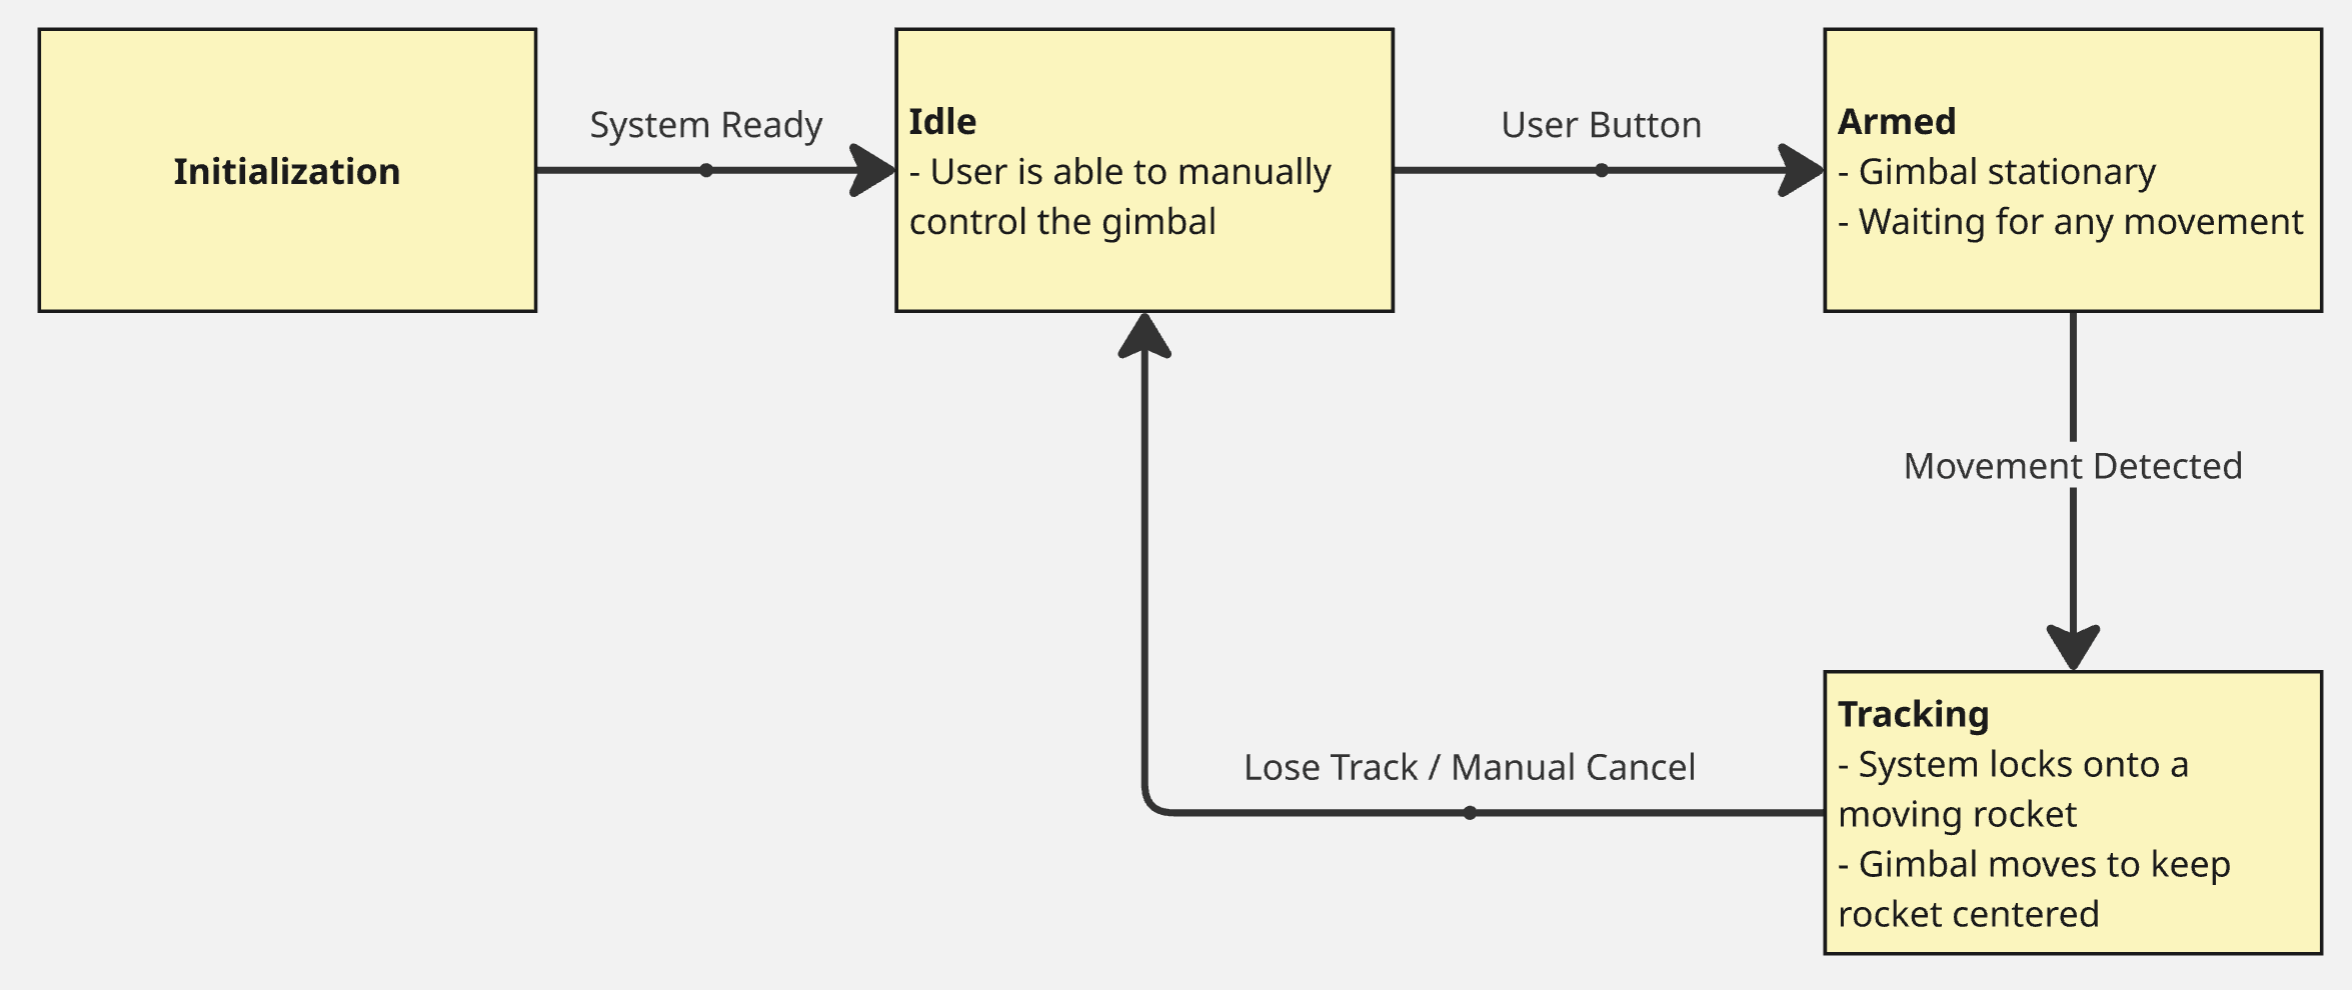
\includegraphics[width=\textwidth,height=\textheight,keepaspectratio]{../Images/state_diagram.png}
  \caption{System State Diagram}
  \label{img:state-diagram}
\end{figure}
\FloatBarrier

\section{Functional Requirements}
\subsection{Functional Requirements}

\begin{itemize}

  \item[FR-SYS-1] \emph{The system must acquire live images or video streams from an
          onboard camera.}\\[2mm]
        {\bf Rationale:} Image acquisition is the first step of the vision-guided pipeline and enables all downstream processing.\\
        {\bf Fit Criterion:} The system successfully captures frames at a usable resolution and passes them to the CV pipeline.\\
        {\bf Priority:} High

  \item[FR-SYS-2] \emph{The system must segment the scene and detect multiple moving
          objects in real time.}\\[2mm]
        {\bf Rationale:} Object detection enables the tracker to identify possible targets for selection and tracking.\\
        {\bf Fit Criterion:} At least two moving objects can be detected simultaneously at $\geq$ 15 FPS on Jetson hardware.\\
        {\bf Priority:} High

  \item[FR-SYS-3] \emph{The system must allow the operator to select a stationary or
          moving object as the target.}\\[2mm]
        {\bf Rationale:} Manual target selection is essential for flexibility, ensuring the system can track user-specified objects.\\
        {\bf Fit Criterion:} Operator input is received and the chosen target is registered by the tracking system.\\
        {\bf Priority:} High

  \item[FR-SYS-4] \emph{The system must continuously estimate the target's position and
          keep it centered in the image.}\\[2mm]
        {\bf Rationale:} Accurate target tracking is the core function of the system to maintain visual lock.\\
        {\bf Fit Criterion:} Target remains within 40 px of frame center at 1080p resolution under smooth motion.\\
        {\bf Priority:} High

  \item[FR-SYS-5] \emph{The system must send real-time pan/tilt commands to the STM32
          microcontroller for gimbal control.}\\[2mm]
        {\bf Rationale:} Gimbal control keeps the target centered physically, extending camera field of view.\\
        {\bf Fit Criterion:} Latency between detected movement and gimbal adjustment is $\leq$ 120 ms.\\
        {\bf Priority:} High

  \item[FR-SYS-6] \emph{The system must detect target occlusion or loss and attempt
          automatic re-acquisition, with manual reselection available.}\\[2mm]
        {\bf Rationale:} Targets may be temporarily obstructed; recovery ensures robustness of the tracking loop.\\
        {\bf Fit Criterion:} The system reacquires a target within 1 second (p95) or allows operator reselection.\\
        {\bf Priority:} Medium

  \item[FR-SYS-7] \emph{The system must provide remote management capabilities for
          operators.}\\[2mm]
        {\bf Rationale:} Remote access supports field deployment and safety by allowing off-device control.\\
        {\bf Fit Criterion:} Operators can access system controls via a web interface on a remote device.\\
        {\bf Priority:} Medium

  \item[FR-SYS-8] \emph{The system must display runtime information including system
          state, FPS, and tracking status.}\\[2mm]
        {\bf Rationale:} Visibility into runtime performance is critical for debugging and operator trust.\\
        {\bf Fit Criterion:} The interface updates system status in real time with FPS $\pm$ 1 frame accuracy.\\
        {\bf Priority:} Medium

  \item[FR-SYS-9] \emph{The system must demonstrate the complete workflow: Acquire
          $\rightarrow$ Detect $\rightarrow$ Select $\rightarrow$ Track $\rightarrow$
          Control.}\\[2mm]
        {\bf Rationale:} The proof-of-concept requires showing the integration of all subsystems working together.\\
        {\bf Fit Criterion:} During demo, the system executes all five stages successfully without manual patching.\\
        {\bf Priority:} High

        % --- Web End Requirements ---
  \item[FR-WEB-1] \emph{The web application must provide a browser-based interface for
          remote management of the system.}\\[2mm]
        {\bf Rationale:} Operators need remote access to safely configure and monitor the system during field testing.\\
        {\bf Fit Criterion:} Operators can log in through a standard browser and access system controls without requiring local installation.\\
        {\bf Priority:} Medium

  \item[FR-WEB-2] \emph{The web application must display runtime status information
          such as system state, frame rate, and tracking status.}\\[2mm]
        {\bf Rationale:} Operators need real-time visibility into performance to make informed decisions and detect issues.\\
        {\bf Fit Criterion:} The dashboard shows current state, FPS, and tracking status, updating within 1 second of backend changes.\\
        {\bf Priority:} Medium

  \item[FR-WEB-3] \emph{The web application must provide controls for manual target
          reselection when automatic tracking fails.}\\[2mm]
        {\bf Rationale:} Manual override enables recovery when auto-reacquisition is unsuccessful.\\
        {\bf Fit Criterion:} When a target is lost, the operator can reselect a target via the web UI and the system resumes tracking within 1 second.\\
        {\bf Priority:} High

  \item[FR-WEB-4] \emph{The web application must allow operators to view the live video
          stream from the camera.}\\[2mm]
        {\bf Rationale:} Visual confirmation of what the system is tracking is necessary for effective operation.\\
        {\bf Fit Criterion:} The live camera feed is viewable in the web interface with end-to-end latency $\leq$ 500 ms relative to the source.\\
        {\bf Priority:} High

  \item[FR-WEB-5] \emph{The web application must allow operators to record video
          sessions for later review.}\\[2mm]
        {\bf Rationale:} Recording supports debugging, validation, and demonstration.\\
        {\bf Fit Criterion:} Operators can start and stop recording from the web UI and access the saved video files afterward.\\
        {\bf Priority:} Medium

  \item[FR-WEB-6] \emph{The web application must provide playback and basic management
          of recorded videos (list, delete, download).}\\[2mm]
        {\bf Rationale:} Reviewing and managing captured sessions supports performance analysis and documentation.\\
        {\bf Fit Criterion:} Operators can select a recording, play it in the web UI, and perform list/delete/download actions.\\
        {\bf Priority:} Low

\end{itemize}
\section{Look and Feel Requirements}
\subsection{Appearance Requirements}
\begin{itemize}[leftmargin=*]
  \item[LFR-AP-1] \emph{The dashboard shall use a light background with high-contrast
          status colors (green = Ready, amber = Armed/Waiting to Activate, red =
          Fault/Lost).}\\ \textbf{Rationale:} Improves readability under bright outdoor
        lighting and noisy environments.\\ \textbf{Fit Criterion:} In a 300-lux outdoor
        setting, users can correctly identify the current status within 2 seconds.

  \item[LFR-AP-2] \emph{Key readouts (FPS, end-to-end latency estimate, tracking
          confidence) shall be visible in the main view without scrolling on a 1080p
          display.}\\ \textbf{Rationale:} Operators need immediate awareness of system
        health and tracking quality.\\ \textbf{Fit Criterion:} On a 1920×1080 monitor,
        all three readouts are simultaneously visible in the primary screen.
\end{itemize}

\subsection{Style Requirements}
\begin{itemize}[leftmargin=*]
  \item[LFR-ST-1] \emph{Units and terminology shall be consistent: speed (°/s),
          resolution (px), frame rate (FPS), distance (km), temperature (°C).}\\
        \textbf{Rationale:} Consistency reduces operator error during high-pressure
        launch operations.\\ \textbf{Fit Criterion:} A style audit of UI readouts finds
        no unit inconsistencies.
\end{itemize}

\section{Usability and Humanity Requirements}
\subsection{Ease of Use Requirements}
\begin{itemize}[leftmargin=*]
  \item[USR-EZ-1] \emph{Cold start to ``Ready'' shall require no more than five
          operator steps; reset time between launches shall be $\leq$ 2 minutes.}\\
        \textbf{Rationale:} Field workflow demands rapid setup/turnaround and minimal
        touches near the pad.\\ \textbf{Fit Criterion:} Operators independently achieve
        average reset time $\leq$ 120 s and $\leq$ 5 steps from cold start to
        ``Ready''.

  \item[USR-EZ-2] \emph{The full operational flow (power on, self-check, arm/identify,
          record, shutdown) shall be executable remotely without visiting the camera
          site.}\\ \textbf{Rationale:} Reduces exposure to hazardous zones.\\ \textbf{Fit
          Criterion:} A complete session is performed via the web-accessible interface
        with zero physical interaction at the camera.
\end{itemize}

\subsection{Personalization and Internationalization Requirements}
\begin{itemize}[leftmargin=*]
  \item[USR-PI-1] \emph{The user interface shall support English and French, switchable
          at runtime.}\\ \textbf{Rationale:} Matches the Canadian event context and
        bilingual stakeholders.\\ \textbf{Fit Criterion:} All primary UI elements are
        localized for EN/FR; language can be switched without restart.
\end{itemize}

\subsection{Learning Requirements}
\begin{itemize}[leftmargin=*]
  \item[USR-LR-1] \emph{A first-time operator shall be able to complete one end-to-end
          run with a toy-rocket scenario within 30 minutes.}\\ \textbf{Rationale:}
        Simulation/training reduces field risk.\\ \textbf{Fit Criterion:} Novice
        operators complete the simulated end-to-end run in $\leq$ 30 minutes.
\end{itemize}

\subsection{Understandability and Politeness Requirements}
\begin{itemize}[leftmargin=*]
  \item[USR-UP-1] \emph{Alerts shall include both the cause and an actionable
          suggestion (e.g., ``Tracking lost: try manual reselect'').}\\
        \textbf{Rationale:} Reduces cognitive load and speeds recovery.\\ \textbf{Fit
          Criterion:} Novice operators can complete recovery flows without assistance in
        usability tests.
\end{itemize}

\subsection{Accessibility Requirements}
\begin{itemize}[leftmargin=*]
  \item[USR-AC-1] \emph{Minimum text size shall be 12\,pt; critical readouts shall be
          $\geq$ 16\,pt; status indicators shall remain distinguishable under common
          color-vision deficiencies.}\\ \textbf{Rationale:} Ensures legibility for
        diverse users and conditions.\\ \textbf{Fit Criterion:} UI passes color-vision
        simulations and font-size checks in a design audit.
\end{itemize}

\section{Performance Requirements}
\subsection{Speed and Latency Requirements}
\begin{itemize}[leftmargin=*]
  \item[PR-SPD-1] \emph{End-to-End live video latency shall be $\leq$ 100\,ms (p95),
          sufficient to enable continuous rocket tracking.}\\ \textbf{Rationale:}
        Assuming hardware performance is adequate, latency budget is dominated by video
        transport and inference.\\ \textbf{Fit Criterion:} Time-synchronized probes
        confirm p95 $\leq$ 100\,ms.

  \item[PR-SPD-2] \emph{AI inference latency per frame shall be $\leq$ 20\,ms (p95) at
          the target resolution on Jetson hardware.}\\ \textbf{Rationale:} Keeps the
        detect–control loop within the motion budget.\\ \textbf{Fit Criterion:}
        Profiling on the target Jetson shows p95 $\leq$ 20\,ms per frame.
\end{itemize}

\subsection{Safety-Critical Requirements}
\begin{itemize}[leftmargin=*]
  \item[PR-SF-1] \emph{Manual override shall preempt automated control at any time.}\\
        \textbf{Rationale:} Ensures a safe fallback in ambiguous or degraded
        conditions.\\ \textbf{Fit Criterion:} In three injected-fault scenarios (loss,
        misdetection, link jitter), override takes effect within 200\,ms.
\end{itemize}

\subsection{Precision or Accuracy Requirements}
\begin{itemize}[leftmargin=*]
  \item[PR-ACU-1] \emph{During flight, the system shall maintain target tracking with
          confidence $\geq 0.5$.}\\ \textbf{Rationale:} Guarantees usable imagery and
        telemetry for analysis.\\ \textbf{Fit Criterion:} Throughout the observable
        flight, tracking is not lost and confidence remains $\geq 0.5$.
\end{itemize}

\subsection{Robustness or Fault-Tolerance Requirements}
\begin{itemize}[leftmargin=*]
  \item[PR-RB-1] \emph{After short occlusion or loss, the system shall attempt auto
          re-acquisition with p95 $\leq$ 1\,s; if unsuccessful, it shall prompt manual
          reselect.}\\ \textbf{Rationale:} Maintains lock through realistic field
        interruptions.\\ \textbf{Fit Criterion:} UI exposes manual reselect on failure;
        re-acquisition succeeds within the stated budget where applicable.
\end{itemize}

\subsection{Capacity Requirements}
\begin{itemize}[leftmargin=*]
  \item[PR-CAP-1] \emph{Local storage shall retain at least five complete launch
          sessions at 1080p@30 before requiring cleanup or offload.}\\
        \textbf{Rationale:} Ensures sufficient retention for review and backup.\\
        \textbf{Fit Criterion:} Five full sessions can be recorded, listed, and played
        back/exported without space errors.
\end{itemize}

\subsection{Scalability or Extensibility Requirements}
\begin{itemize}[leftmargin=*]
  \item[PR-SCL-1] \emph{The inference stack shall support ONNX deployment and TensorRT
          optimization.}\\ \textbf{Rationale:} Preserves portability and performance
        tuning headroom.\\ \textbf{Fit Criterion:} Models load and run via ONNX;
        TensorRT engine builds succeed for the target GPU.
\end{itemize}

\subsection{Longevity Requirements}
\begin{itemize}[leftmargin=*]
  \item[PR-LNG-1] \emph{System endurance shall be $\geq$ 6 hours of continuous
          operation; daily operating cost shall be $<\$100$.}\\ \textbf{Rationale:}
        Matches event-day duty cycles and budget constraints.\\ \textbf{Fit Criterion:}
        Power tests show $\geq$ 6 hours; cost worksheet shows $<\$100$/day.
\end{itemize}

\section{Operational and Environmental Requirements}
\subsection{Expected Physical Environment}
\begin{itemize}[leftmargin=*]
  \item[OER-ENV-1] \emph{Operating temperature range shall be -10\,°C to 45\,°C;
          relative humidity up to 90\%.}\\ \textbf{Rationale:} Outdoor launch sites
        present cold, heat, and moisture.\\ \textbf{Fit Criterion:} Climatic tests at
        endpoints for 2 hours show stable operation without thermal shutdown.
\end{itemize}

\subsection{Wider Environment Requirements}
\begin{itemize}[leftmargin=*]
  \item[OER-WE-1] \emph{The enclosure and cabling shall meet IP65 or better for dust
          protection and weather resistance.}\\ \textbf{Rationale:} Wind, dust, and
        precipitation are common on ranges.\\ \textbf{Fit Criterion:} Provide test
        certificates or equivalent field test records meeting IP65 criteria.
\end{itemize}

\subsection{Requirements for Interfacing with Adjacent Systems}
\begin{itemize}[leftmargin=*]
  \item[OER-INT-1] \emph{Provide an HDMI program feed and an IP stream compatible with
          common switchers/encoders; remote control range shall be $\geq$ 100\,m.}\\
        \textbf{Rationale:} Integrates with broadcast rigs and supports distant safe
        operation.\\ \textbf{Fit Criterion:} Verified ingest into OBS/capture cards;
        stable remote control over a measured 100\,m link.
\end{itemize}

\subsection{Productization Requirements}
\begin{itemize}[leftmargin=*]
  \item[OER-PZ-1] \emph{The field kit shall support integrated cabling and allow
          deployment/teardown within 15 minutes.}\\ \textbf{Rationale:} Minimizes
        schedule impact between flights.\\ \textbf{Fit Criterion:} Drills show average
        deploy or teardown time $\leq$ 15 minutes.
\end{itemize}

\subsection{Release Requirements}
\begin{itemize}[leftmargin=*]
  \item[OER-REL-1] \emph{Each public release shall include a parameter sheet and links
          to system, network, and support documentation.}\\ \textbf{Rationale:} Speeds
        onboarding of new crew and stakeholders.\\ \textbf{Fit Criterion:} Release
        bundle contains the parameter sheet and referenced chapters.
\end{itemize}

\section{Maintainability and Support Requirements}
\subsection{Maintenance Requirements}
\begin{itemize}[leftmargin=*]
  \item[MSR-MA-1] \emph{Thresholds for FPS, latency, and confidence shall be adjustable
          via configuration or admin UI without recompilation.}\\ \textbf{Rationale:}
        Facilitates tuning across sites and hardware.\\ \textbf{Fit Criterion:} Changes
        take effect without backend restart and within 60 seconds.
\end{itemize}

\subsection{Supportability Requirements}
\begin{itemize}[leftmargin=*]
  \item[MSR-SP-1] \emph{Exportable logs shall include frame timestamps, tracking error,
          and event markers (e.g., ignition, staging, chute).}\\ \textbf{Rationale:}
        Enables post-flight analysis and issue triage.\\ \textbf{Fit Criterion:} After
        a launch, CSV/JSON with the three fields is available for download.
\end{itemize}

\subsection{Adaptability Requirements}
\begin{itemize}[leftmargin=*]
  \item[MSR-AD-1] \emph{The gimbal abstraction layer shall support the gimbal provided
          by the rocket team without changes to core tracking code.}\\ \textbf{Fit
          Criterion:} The gimbal control passes pan/tilt/zoom command and calibration
        tests.
\end{itemize}

\section{Security Requirements}
\subsection{Access Requirements}
\begin{itemize}[leftmargin=*]
  \item[SEC-AC-1] \emph{Remote management UI shall require authentication; three
          consecutive failed logins shall trigger a lockout of at least 5 minutes.}\\
        \textbf{Rationale:} Protects control paths exposed over the network.\\
        \textbf{Fit Criterion:} Black-box tests confirm lockout after three failed
        attempts.
\end{itemize}

\subsection{Integrity Requirements}
\begin{itemize}[leftmargin=*]
  \item[SEC-IN-1] \emph{Configurations and logs shall include checksums or signatures;
          control commands shall use authenticated channels.}\\ \textbf{Rationale:}
        Prevents tampering and unauthorized actuation.\\ \textbf{Fit Criterion:}
        Tampering is detected; unauthenticated devices cannot issue PTZ commands.
\end{itemize}

\subsection{Privacy Requirements}
\begin{itemize}[leftmargin=*]
  \item[SEC-PV-1] \emph{Access to recordings and logs shall be role-based
          (Operator/Analyst/Admin) with least-privilege defaults.}\\ \textbf{Rationale:}
        Aligns access with duties while limiting exposure.\\ \textbf{Fit Criterion:}
        Role matrix is enforced in acceptance tests.
\end{itemize}

\subsection{Audit Requirements}
\begin{itemize}[leftmargin=*]
  \item[SEC-AU-1] \emph{Audit logs shall record login, configuration changes, manual
          overrides, and deletion of recordings.}\\ \textbf{Rationale:} Supports
        accountability and incident reconstruction.\\ \textbf{Fit Criterion:} Each
        audited event contains actor, timestamp, action, and target.
\end{itemize}

\subsection{Immunity Requirements}
\begin{itemize}[leftmargin=*]
  \item[SEC-IM-1] \emph{On communication loss or heavy jitter, the system shall enter a
          safe-hold state and avoid hazardous motion; upon recovery it shall reconnect
          smoothly.}\\ \textbf{Rationale:} Prevents unsafe behavior under network
        faults.\\ \textbf{Fit Criterion:} Injected outages of $\geq$ 10 seconds cause
        no dangerous actuation; control recovers automatically.
\end{itemize}

\section{Cultural Requirements}
\begin{itemize}[leftmargin=*]
  \item[CUL-1] \emph{The product shall suit university competition settings: bilingual
          EN/FR support and neutral, non-biased terminology in UI and logs.}\\
        \textbf{Rationale:} Inclusive collaboration across teams and organizers.\\
        \textbf{Fit Criterion:} Terminology review finds no culturally biased phrasing;
        EN/FR toggle is available.
\end{itemize}

\section{Compliance Requirements}
\subsection{Legal Requirements}
\begin{itemize}[leftmargin=*]
  \item[CMP-LG-1] \emph{Recording, streaming, and data retention shall follow event and
          venue policies regarding image rights and privacy.}\\ \textbf{Rationale:}
        Ensures lawful operation at competitions and ranges.\\ \textbf{Fit Criterion:}
        A pre-event compliance checklist is reviewed and approved by the organizer.
\end{itemize}

\subsection{Standards Compliance Requirements}
\begin{itemize}[leftmargin=*]
  \item[CMP-ST-1] \emph{Networking/interfaces shall use standard IP/HTTP and common
          video formats; AI deployment shall be compatible with ONNX and TensorRT.}\\
        \textbf{Rationale:} Interoperability with broadcast tools and GPU inference
        stacks.\\ \textbf{Fit Criterion:} Ingest succeeds in mainstream
        encoders/capture tools; ONNX models load and run with TensorRT optimization.
\end{itemize}

\section{Open Issues}
\lips

\section{Off-the-Shelf Solutions}
\subsection{Ready-Made Products}
\lips
\subsection{Reusable Components}
\lips
\subsection{Products That Can Be Copied}
\lips

\section{New Problems}
\subsection{Effects on the Current Environment}
\lips
\subsection{Effects on the Installed Systems}
\lips
\subsection{Potential User Problems}
\lips
\subsection{Limitations in the Anticipated Implementation Environment That May
  Inhibit the New Product}
\lips
\subsection{Follow-Up Problems}
\lips

\section{Tasks}
\subsection{Project Planning}
\lips
\subsection{Planning of the Development Phases}
\lips

\section{Migration to the New Product}
\subsection{Requirements for Migration to the New Product}
\lips
\subsection{Data That Has to be Modified or Translated for the New System}
\lips

\section{Costs}
\lips
\section{User Documentation and Training}
\subsection{User Documentation Requirements}
\lips
\subsection{Training Requirements}
\lips

\section{Waiting Room}
\lips

\section{Ideas for Solution}
\lips

\newpage{}
\section*{Appendix --- Reflection}

The purpose of reflection questions is to give you a chance to assess your own
learning and that of your group as a whole, and to find ways to improve in the
future. Reflection is an important part of the learning process.  Reflection is
also an essential component of a successful software development process.  

Reflections are most interesting and useful when they're honest, even if the
stories they tell are imperfect. You will be marked based on your depth of
thought and analysis, and not based on the content of the reflections
themselves. Thus, for full marks we encourage you to answer openly and honestly
and to avoid simply writing ``what you think the evaluator wants to hear.''

Please answer the following questions.  Some questions can be answered on the
team level, but where appropriate, each team member should write their own
response:


\begin{enumerate}
  \item What went well while writing this deliverable?
  \item What pain points did you experience during this deliverable, and how did you
        resolve them?
  \item How many of your requirements were inspired by speaking to your client(s) or
        their proxies (e.g. your peers, stakeholders, potential users)?
  \item Which of the courses you have taken, or are currently taking, will help your
        team to be successful with your capstone project.
  \item What knowledge and skills will the team collectively need to acquire to
        successfully complete this capstone project? Examples of possible knowledge to
        acquire include domain specific knowledge from the domain of your application,
        or software engineering knowledge, mechatronics knowledge or computer science
        knowledge. Skills may be related to technology, or writing, or presentation, or
        team management, etc. You should look to identify at least one item for each
        team member.
  \item For each of the knowledge areas and skills identified in the previous question,
        what are at least two approaches to acquiring the knowledge or mastering the
        skill? Of the identified approaches, which will each team member pursue, and
        why did they make this choice?
\end{enumerate}


\end{document}